\documentclass[11pt, a4paper]{article}

\usepackage[T1]{fontenc}
\usepackage[utf8]{inputenc}
\usepackage[norsk]{babel}
\usepackage{amsmath}
\usepackage{amsfonts}
\usepackage{amssymb}
\usepackage{graphicx}
\usepackage{verbatim}
\usepackage{caption}
\usepackage{subcaption}
\usepackage{subfig}
\usepackage{float}
\usepackage{program}
\usepackage{commath}

\begin{document}

\begin{titlepage}
  
  \title{\normalsize FYS1120 Elektromagnetisme 2014\\
  \vspace{10mm}
  \huge Oblig 2\\
  \vspace{10mm}
  \normalsize{\bf Partiklar i elektriske og magnetiske felt.}}

  \author{Øyvind Sigmundson Schøyen}

\end{titlepage}

\maketitle

\begin{figure}[H]
  \centering
  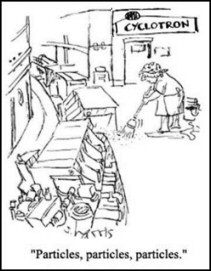
\includegraphics[width=150px]{cyclotron.jpg}
\end{figure}

\newpage
  \tableofcontents
\newpage

\section{Partikkel i elektrisk felt}
  Det er ikkje oppført i denne oppgåva om me skal sjå vekk frå gravitasjonskrafta, men eg har ikkje tatt ho med i utrekningane. Dette grunna då me nyttar dimensjonslause variablar som eg 
  ikkje kjenner konstantane til.

  \begin{figure}[H]
    \centering
    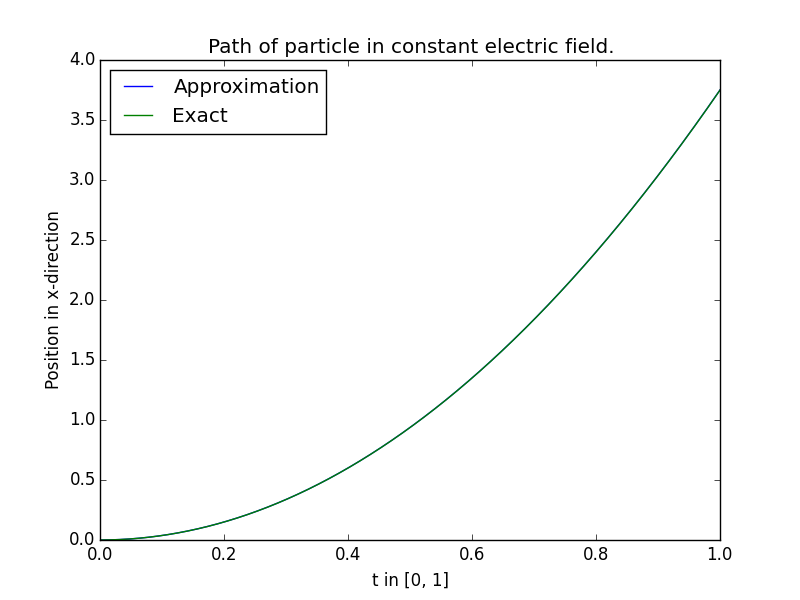
\includegraphics[width=300px]{A.png}
    \caption{I dette plottet ser me plott over posisjonen til partikkelen i $x$-retning mot 
    tid samt den analytiske løysninga som ligg over.
    Me kan sjå at grunna konstant akselerasjon vil me ha ein lineær hastighet. Difor må 
    posisjonen gå som ein kvadratisk funksjon. Dette vil hjelpe oss med å verifisere den 
    analytiske løysninga.}
  \end{figure}
  Når me skal utleie den analytiske løysninga vil me nytte Newtons andre lov i lag med uttrykket for krafta i eit $\mathbf{E}$-felt. Då får me
  \begin{align*}
    \mathbf{F} = q\mathbf{E} = m\mathbf{a}(t) \qquad \Rightarrow \qquad \mathbf{a}(t) = \frac{q}{m}\mathbf{E}.
  \end{align*}
  No vil me integrere med hensyn på tid. Me har heile vegen eit bestemt integral kor me byrjar på $t = 0$. Då får me
  \begin{align*}
    \mathbf{v}(t) = \int_0^t\mathbf{a}(t) \ dt = \int_0^t \frac{q}{m}\mathbf{E} \ dt = \frac{q}{m}\mathbf{E}t.
  \end{align*}
  Me integrerer ei gong til for å finne posisjonen.
  \begin{align*}
    \mathbf{r}(t) = \int_0^t\mathbf{v}(t) \ dt = \int_0^t \frac{q}{m}\mathbf{E}t \ dt = \frac{1}{2}\frac{q}{m}\mathbf{E}t^2.
  \end{align*}
  Resultatet av denne ser me i Figur 1.

  \begin{figure}[H]
    \centering
    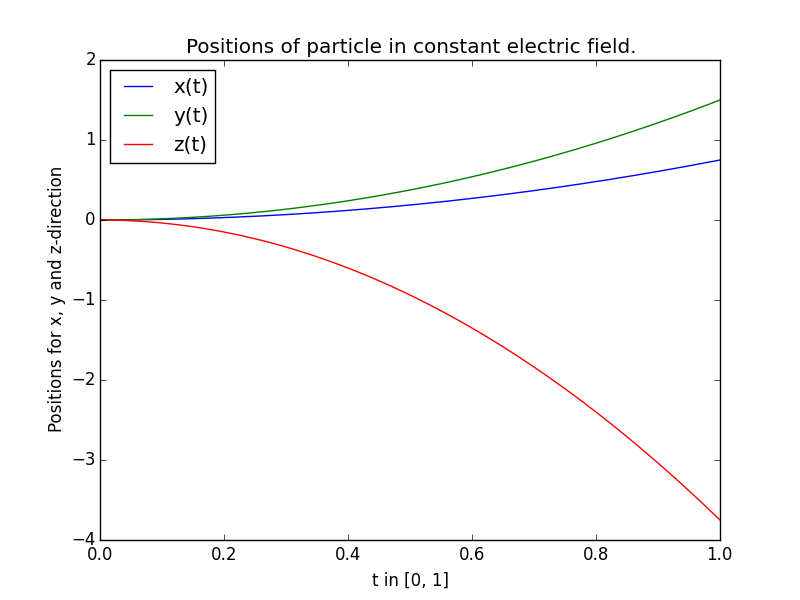
\includegraphics[width=300px]{C1.png}
    \caption{Her ser me plott for posisjonane i $x$, $y$ og $z$-retning mot tid.}
  \end{figure}

  \begin{figure}[H]
    \centering
    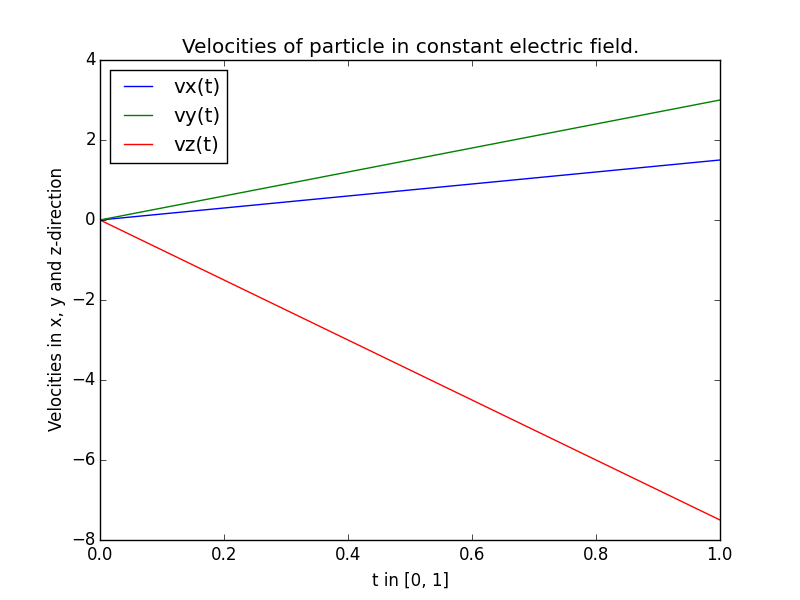
\includegraphics[width=300px]{C2.png}
    \caption{Her ser me plott for hastighetane i $x$, $y$ og $z$-retning mot tid. Siden $\mathbf{E}$-feltet har komponenta i alle tre retningane har me ein konstant akselerasjon 
    som gjer oss ein lineært aukande hastighet for alle retningane.}
  \end{figure}
  Me kan sjå at dette vil bli ei ballistisk rørsle då partikkelen vil ha ei konstant aukande fart. Resultatet av dette gjer oss ein posisjon som går som ein andregradsfunksjon.
  Partikkelen vil difor bli ``skutt ut''.

  \begin{figure}[H]
    \centering
    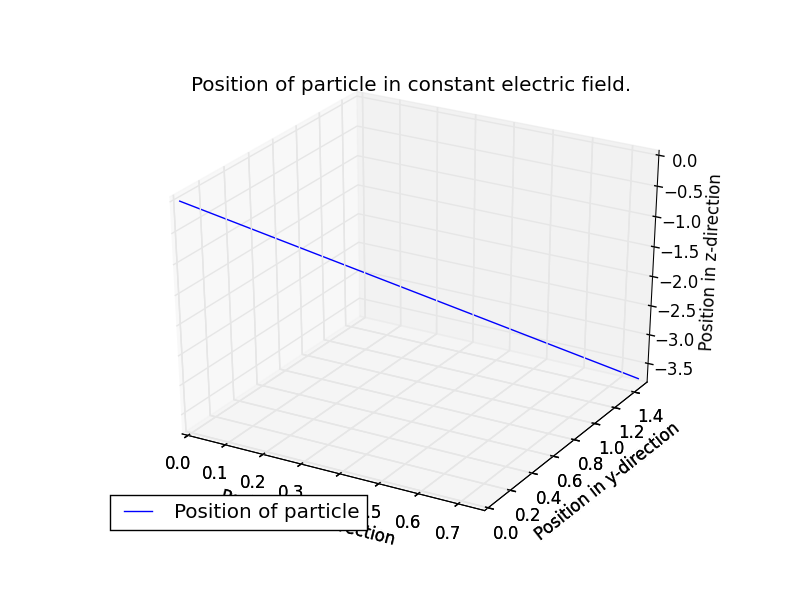
\includegraphics[width=300px]{D.png}
    \caption{Her vil me sjå korleis partikkelen forflyttar seg i rommet. Me ser derimot ikkje korleis han auker i hastighet. Viss me hadde vist dette som ein film mot tid ville me 
    sett korleis avstanden mellom kvart sekund ville auke.}
  \end{figure}


\newpage
\section{Partikkel i magnetisk felt}

  \begin{figure}[H]
    \centering
    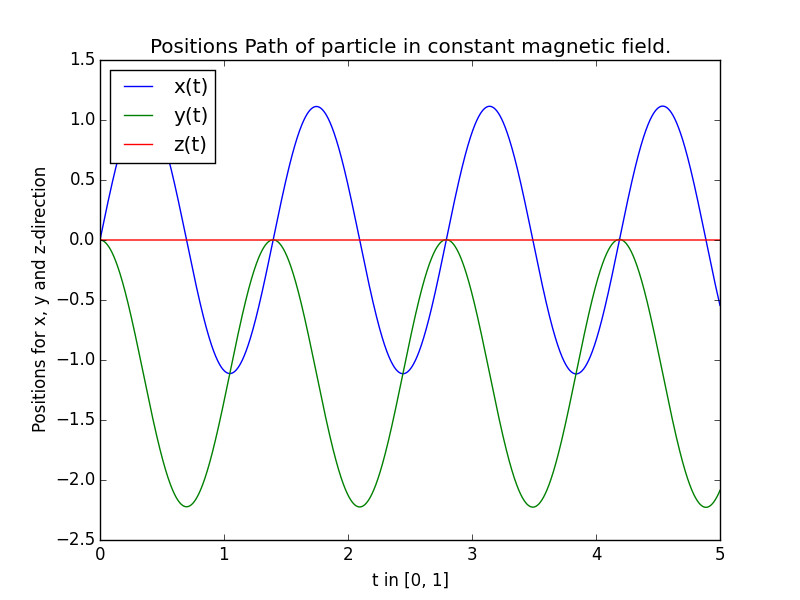
\includegraphics[width=300px]{2A1.png}
    \caption{Her ser me eit plott over posisjonen til partikkelen i $x$, $y$ og $z$-retning mot tid. Magnetfeltet gjer oss ei kraft som virker inn mot sentrum av ein sirkel. 
    Me får difor svingningar for $x$ og $y$-retning då partikkelen beveger seg i ein sirkel i $xy$-planet. I $z$-retning har me derimot ingen kraftkomponent og partikkelen endrar ikkje 
    posisjon.}
  \end{figure}

  \begin{figure}[H]
    \centering
    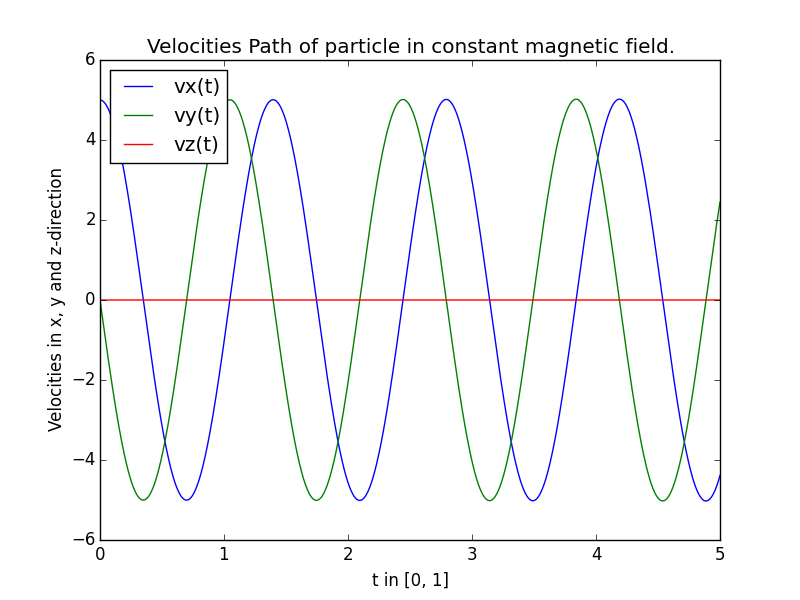
\includegraphics[width=300px]{2A2.png}
    \caption{Plottet viser oss hastighetane i $x$, $y$ og $z$-retning mot tid. Me får liknande svingningar for hastighetane som for posisjonane.}
  \end{figure}

  \begin{figure}[H]
    \centering
    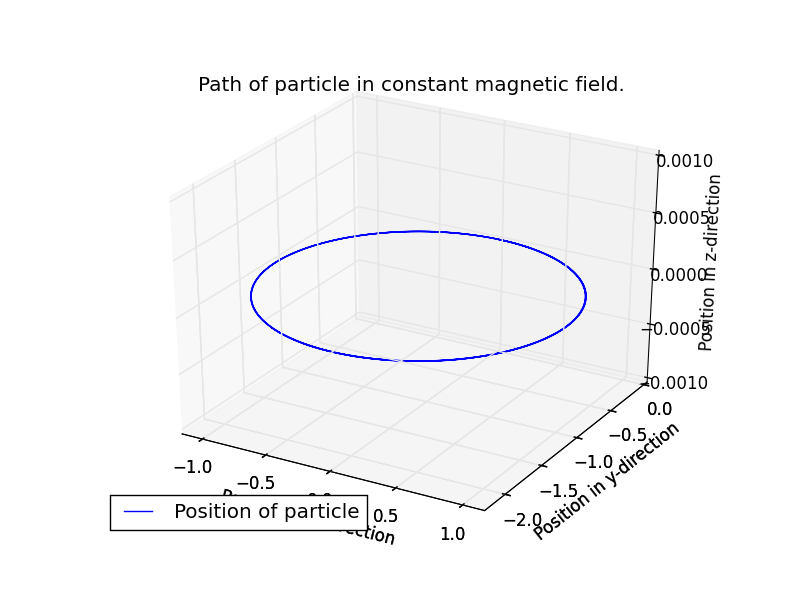
\includegraphics[width=300px]{2A3.png}
    \caption{Her kjem det tydeleg fram korleis partikkelen beveger seg i ein sirkelbane i magnetfeltet. Dette fordi partikkelen vil ha ein konstant kraftkomponent inn mot sirkelen.
    Me får då ein sentripetalakselerasjon som vil trekke partikkelen rundt i ein sirkelbane.}
  \end{figure}

  Programmet $\texttt{Oppgave2.py}$ gjer oss utskrifta
  \begin{center}
    \input{utskrift.txt}
  \end{center}
  Måten dette vert rekna ut vil bli forklart i programmet til slutt i besvarelsen. \\ \\

  For å finne syklotronfrekvensen nyttar me uttrykket for krafta frå det magnetiske feltet i lag med Newtons andre lov.
  \begin{align*}
    \mathbf{F}_B = q\left( \mathbf{v} \times \mathbf{B} \right) = m\mathbf{a}.
  \end{align*}
  Siden det magnetiske feltet kun virker i $z$-retning og me er interesserte i den tangensielle hastigheten vil me jobbe med uttrykket
  \begin{align*}
    F_B = qvB = ma = m\frac{v^2}{r},
  \end{align*}
  kor me i siste ledd har brukt at sentripetalakselerasjonen er gjeve ved
  \begin{align*}
    a = \frac{v^2}{r}.
  \end{align*}
  Då vil me få
  \begin{align*}
    qvB = m\frac{v^2}{r} \qquad \Rightarrow \qquad v = \frac{qrB}{m}.
  \end{align*}
  No nyttar me at vinkelhastigheten er gitt ved 
  \begin{align*}
    \omega = \frac{v}{r} \qquad \Rightarrow \qquad v = r\omega.
  \end{align*}
  Det gjer oss
  \begin{align*}
    \omega = \frac{qB}{m}.
  \end{align*}
  Omlaupsperioden $T$ er gjeve ved 
  \begin{align*}
    T = \frac{2\pi}{\omega}.
  \end{align*}
  Då fylgjer det at
  \begin{align*}
    T = \frac{2\pi}{w} = \frac{2\pi m}{qB}.
  \end{align*}
  Me vil då få ein omlaupsperiode på 
  \begin{align*}
    T = \frac{2\pi (2)}{(3)(3)} \approx 1.3962.
  \end{align*}
  Dette er veldig nærme det me får frå det numeriske resultatet. Eventuelle feil vil kome frå numerisk avrunding då me på datamaskinen ikkje klarer å representere flyttal eksakt. Det vil 
  og vere vanskeleg å køyre ein eksakt if-test med flyttal.

  \begin{figure}[H]
    \centering
    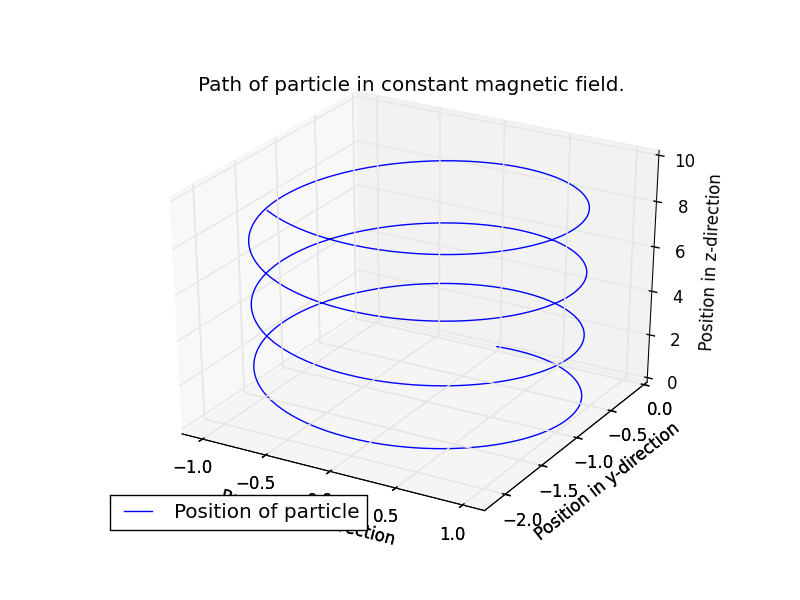
\includegraphics[width=300px]{2A4.png}
    \caption{Plottet vil her danne ein spiral som flyttar seg i positiv $z$-retning då me ikkje har noko tyngdekraft som motvirkar. I tillegg vil all krafta frå det magnetiske 
    feltet virke i $xy$-planet og vil difor ikkje endre på startverdien til $\mathbf{v}$ i $z$-retning.}
  \end{figure}







\newpage
\section{Partikkel i syklotron}

  \begin{figure}[H]
    \centering
    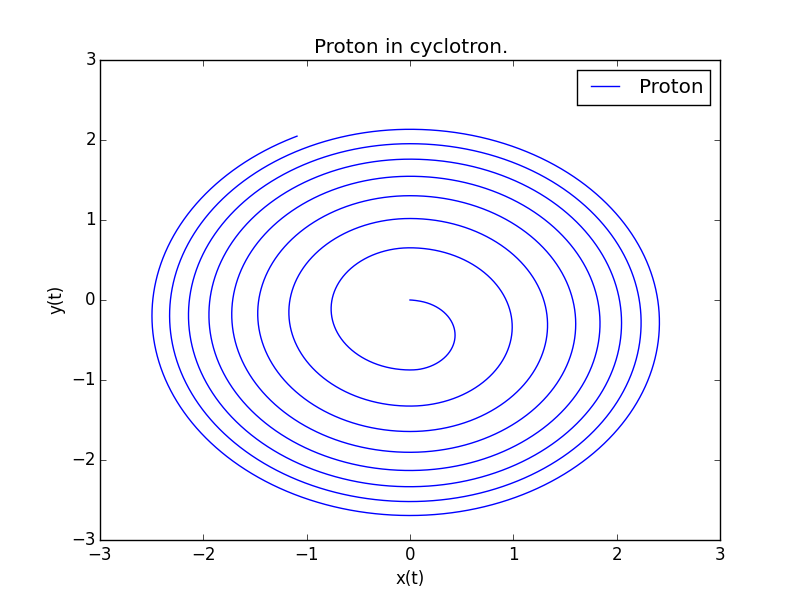
\includegraphics[width=300px]{3A.png}
    \caption{Me ser tydeleg korleis protonet flyttar seg utover i syklotronen etter som tida auker.}
  \end{figure}
  Radien auker derimot ikkje jamnt. Dette kjeme frå det faktum at partikkelen nyttar mindre og mindre tid mellom D'ane, kor protonet vert tilførd meir energi, samanlikna med tid brukt 
  inne i D'ane. % Prøv å utdyp

  \begin{figure}[H]
    \centering
    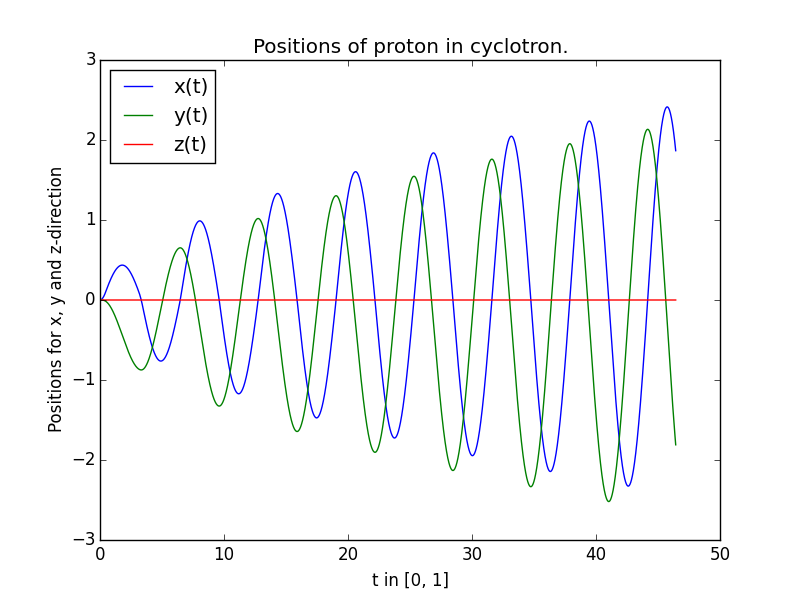
\includegraphics[width=300px]{3A1.png}
    \caption{BLA}
  \end{figure}

  \begin{figure}[H]
    \centering
    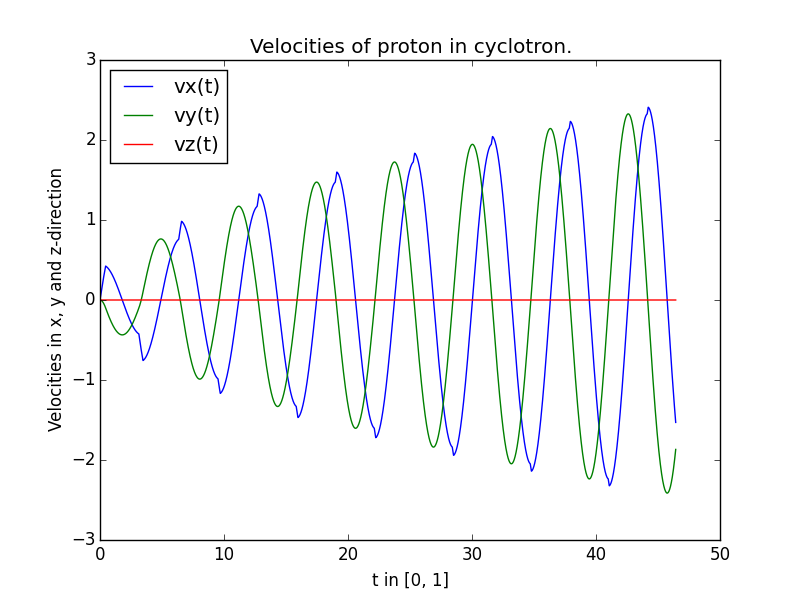
\includegraphics[width=300px]{3A2.png}
    \caption{BLABLA}
  \end{figure}

  Farten partikkelen forlater syklotronen med vert rekna ut i programmet $\texttt{Oppgave3.py}$. Dette vil bli forklart ved programma. % DO THIS!
  Programmet gjer oss utskrifta
  \begin{center}
    \input{utskrift2.txt}
  \end{center}
  Dette seier oss lite då $v$ er dimensjonslaus. Når me no rekner ut energien vil me kunne finne eit uttrykk for hastigheta. \\ \\
  For å finne eit uttrykk for den kinetiske energien nyttar me igjen Newtons andre lov kor me ser sentripetalakselerasjonen og hastigheten i tangensiell retning.
  \begin{align*}
    v = \frac{qrB}{m}
  \end{align*}
  Dette setter me inn i uttrykket for kinetisk energi gjeve ved
  \begin{align*}
    E_k = \frac{1}{2}mv^2.
  \end{align*}
  Me får
  \begin{align*}
    E_k = \frac{1}{2}m\left( \frac{qrB}{m} \right)^2 = \frac{1}{2}\frac{\left( qrB \right)^2}{m}.
  \end{align*}
  Me setter inn verdiane for eit proton som me finn i ein tabell, $m_P = 1.673\times10^{-27}$ kg, $q = 1.602\times10^{-19}$ C.
  \begin{align*}
    E_k &= \frac{1}{2}\frac{\left( (1.602\times10^{-19}\text{ C})(1 \text{ T})(1\text{ m}) \right)^2}{1.673\times10^{-27}\text{ kg}} \\
    &\approx 7.67\times10^{-12}\text{ J} \\
    &\approx 47.87 \text{ MeV}.
  \end{align*}
  Viss me no setter dette lik det klassiske uttrykket for kinetisk energi finner me at protonet har ei hastighet på 
  \begin{align*}
    v \approx 0.32\text{ c},
  \end{align*}
  kor c er lysfarta. Dette er ei såpass høg hastighet at me ikkje kan neglisjere den relativistiske effekten på hastigheta. \\ \\

  For å rekne ut antal rundar som trengs vil me finne eit forholdstal mellom $E_k$ og tilført energi $U$. Dette vil vere gjeve ved
  \begin{align*}
    E_k = nU,
  \end{align*}
  kor $n$ vil vere antal rundar. Siden protonet opplever ei energitilføring to gonger per runde vil me få formelen
  \begin{align*}
    n = \frac{E_k}{2U}.
  \end{align*}
  Då har me at $U$ er gjeve ved
  \begin{align*}
    U = qV
  \end{align*}.
  Eg antar at ein eksperimentelt tilgjengeleg spenning vil vere $V = 50$ kV. Det gjer oss
  \begin{align*}
    U &= qV = (1.602\times10^{-19} \text{ C})(50\times10^3\text{ V}) \\
    &\approx 8.01\times10^{-15}\text{ J}.
  \end{align*}
  Då finner me antal rundar til å vere
  \begin{align*}
    n &= \frac{7.67\times10^{-12}\text{ J}}{2(8.01\times10^{-15}\text {J}} \\
    &\approx 479 \text{ Rundar}.
  \end{align*}
  Frekvensen er definert som ``ein runde per sekund''. Det gjer oss
  \begin{align*}
    f &= \frac{1}{T} = \frac{qB}{2\pi m} \\
    &= \frac{(1.602\times10^{-19}\text{ C})(1 \text{ T})}{2\pi (1.673\times10^{-27}\text{ kg})} \\
    &\approx 15.2\text{ MHz}.
  \end{align*}








\newpage

\section{Programma}
  \subsection{Oppgave1.py}
    \verbatiminput{Oppgave1.py}
  \subsection{Oppgave2.py}
    \verbatiminput{Oppgave2.py}
  \subsection{Oppgave3.py}
    \verbatiminput{Oppgave3.py}


\end{document}
